\documentclass[a4paper,10pt,twocolumn,twoside]{article}

\usepackage[brazilian]{babel}
\usepackage[utf8]{inputenc}
\usepackage[T1]{fontenc}
\usepackage{times}
\usepackage[numbers]{natbib}
\usepackage{hyperref}
\usepackage{caption}
\usepackage{amsfonts}
\usepackage{amsmath}
\usepackage{amssymb}
\usepackage{subfig}
\usepackage{graphicx}
\usepackage{epsfig}
\usepackage{epstopdf}
\usepackage{comment}
\usepackage{array}
\usepackage{booktabs}
\usepackage{multirow}
\usepackage{url}
\usepackage{tabularx}
\usepackage{tabulary}
\usepackage[export]{adjustbox}
\usepackage{algorithm}
\usepackage[noend]{algpseudocode}
%\usepackage[sort,nocompress]{cite}
\usepackage{geometry}
\geometry{top=2.1cm,bottom=1.8cm,left=2.1cm,right=2.1cm}
\usepackage[colorinlistoftodos]{todonotes}

\providecommand{\keywords}[1]{\textbf{\textit{Palavras-Chaves: }} #1}

\begin{document}

\tolerance=999
\sloppy

\title{
A Computational Tool for Geometric Characterization of Fractures
}

\author{
Let\'icia da Silva Bomfim, Helio Pedrini\\
Institute of Computing, University of Campinas (UNICAMP) \\
Campinas, SP, Brazil }

\date{}

\maketitle

\begin{abstract}

\noindent Fraturas são estruturas que podem ser encontradas no interior de uma rocha  e, através de suas características, é possível avaliar e quantificar os atributos os indicadores que influenciam  o volume de fluidos que fluem ao longo do reservatório. Com base nessa premissa, desenvolvemos uma ferramenta que analisa imagens de microtomografia computadorizada extraindo características das fraturas como densidade, tamanho, angulação e tipo. Para essa análise, metodologias e técnicas foram desenvolvidas para avaliar a estrutura dos contornos apresentados no através da segmentação dos dados de entrada. Com isso, foi possível caracterizar a sua geometria e obter uma visualização tridimensional (3D) das estruturas extraídas. Assim, este artigo apresenta as técnicas e os algoritmos que foram desenvolvidas para a caracterização desses importantes parâmetros, principalmente para à área de caracterização de reservatórios e de fluido, evitando assim, uma análise destrutiva da amostra. Além disso,  um ambiente único foi desenvolvido para o tratamento e a análise das imagens, sendo capaz de auxiliar o pesquisador da área especifica de rocha e fluidos, a reduzir as incertezas inerentes a caracterização e, consequentemente, melhorar a confiabilidade no modelo e o poder de decisão ao longo da vida produtiva de um campo. 

\end{abstract}

\begin{keywords}
Porosidade. Fraturas. Microtomografia. Análise. Caracterização.
\end{keywords}

\section{Introdução}
\label{sec:introducao}


Muitos reservatórios de petróleo, geotermais e de abastecimento de água são formados em rochas fraturadas~\cite{national1996rock}. Isso fornece uma grande importância ao estudo das estruturas internas, como poros e fraturas, encontradas nas rochas, pois, por meio delas são formados caminhos que proporcionam a propagação e condução dessas substâncias químicas.


As fraturas são os planos ao longo dos quais o estresse causou perda parcial de coesão na rocha. É uma superfície plana relativamente lisa, representando
plano de fraqueza (descontinuidade)~\cite{singhal2010applied} e sua existência pode causar ou impedir um fluxo de fluido entre elas. 

Assim, a determinação de sua geometria é de suma importância para alimentar simuladores de fluxo, que se utilizam de modelos matemáticos de escoamento em meio poroso para descrever o fenômeno físico do fluxo de massa e/ou energia, a partir de parâmetros macroscópicos. 

Para ter contato com essas estruturas, torna-se necessário coletar um fragmento de rocha que possibilite o estudo dos parâmetros macroscópicos que represente um reservatório. Para isso, extrações são realizadas afim de coletar amostras de rochas, também chamadas de testemunhos, das profundezas da terra. Porém, como esse processo é extremamente árduo e oneroso, utilizar métodos que não agridam a integridade da amostra é o melhor caminho para preservar e perpetuar o material colhido.

Outro ponto que reforça a necessidade de métodos não destrutivos é a dificuldade de análise da amostra para obter as suas propriedades. \citet{jing2007fundamentals} afirmaram que uma explícita representação de todas as fraturas individuais podem ser obtidas diretamente para a geração de um modelo determinístico para análise ou projeto, mas que esse processo, quando feito manualmente, é impraticável devido à grande quantidade de fraturas com diferentes distribuições.

Dessa forma, a técnica de microtomografia computadorizada vem sendo empregada a fim de evitar que as características permo-porosas sejam modificadas a medida que experimentos laboratoriais são realizados, favorecendo a durabilidade e originalidade da amostra, além de permitir uma análise mais profunda do que um estudo manual oferece, visto que técnicas de processamento de imagens podem ser aplicadas nas imagens obtidas. Não veio para substituindo os experimentos laboratoriais mas sim para complementando-os.


Como exemplo, a Figura~\ref{fig:microct} apresenta uma amostra de rocha com a presença de fratura.

\begin{figure}[!htb]
\centering
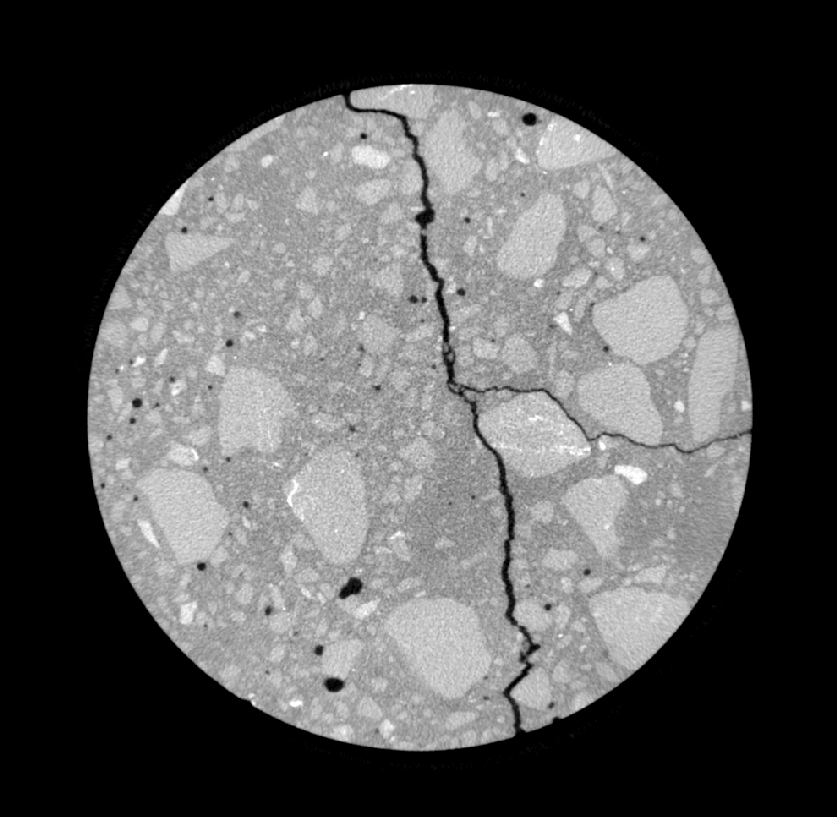
\includegraphics[width=0.27\textwidth]{Figuras/fratura.png} \hspace*{0.1cm}

\caption{imagem de rocha carbonática com a presença de fraturamento  Fonte:~\cite{dataFracture1}.}
\label{fig:microct}
\end{figure}

Com base nisso, a partir do grupo de imagens tomográficas geradas através de uma amostra, desenvolvemos um algoritmo que atua de forma bidimensional (2D) em seu processamento, visando identificar as fraturas presentes, e caracterizá-las de acordo com a sua geometria. Esse processo se dá inicialmente pela segmentação, onde além de extrair as estruturas, também gera uma imagem "máscara" que delimita a área de interesse da rocha, permitindo a análise dos componentes detectados.

Dessa forma, além de analisar cada fratura de forma individual, realiza-se também uma análise geral da fatia 2D em processamento, em que os dados a respeito do conjunto completo de fraturas encontradas são analisadas a fim de quantifica-las em número, densidade (em três diferentes formas: 2D e 3D) e percentagens relativas à inclinação e à forma. 

Este artigo está organizado como segue. Na Seção~\ref{sec:estado_arte}, um referencial teórico apresentará conceitos relevantes sobre as características a serem extraídas das fraturas e dos poros. Na Seção~\ref{sec:metodo}, a metodologia de desenvolvimento do algoritmo e sua interface é descrita. Na Seção~\ref{sec:resultados}, os resultados experimentais são apresentados e discutidos. Finalmente, as conclusões e propostas para trabalhos futuros são descritas na Seção~\ref{sec:conclusoes}.

\section{Estado da Arte}
\label{sec:estado_arte}

Nesta seção, contextualizaremos os trabalhos recentes na área de análise de rochas provenientes de Microtomografia Computadorizada e, em seguida, abordaremos as características que serão avaliadas em cada estrutura (poros e fraturas). 

\subsection{Trabalhos Relacionados}


A análise de rochas carbonáticas é uma prática muito comum no estudo do fluxo de fluidos. Uma das formas mais antigas e ainda comumente utilizadas devido a sua precisão é a injeção de fluidos não-molhantes. Segundo Lucia~\cite{lucia2007carbonate}, o método mais preciso é a expansão de gás hélio, em que uma amostra seca é colocada em uma câmara de volume conhecido e a pressão é calculada com e sem a amostra mantendo-se o volume de gás constante, tal que a diferença de pressão indicará o volume dos poros.

O uso da injeção de mercúrio também é utilizada para esse fim, entretanto, o processo pode gerar a destruição da amostra e somente é empregado em circunstâncias especiais. O teste é feito introduzindo a amostra em um recipiente dotado de um capilar, em que a amostra se encontra em ambiente de vácuo. O mercúrio é injetado no recipiente preenchendo também o capilar para que adentre as fissuras e os macroporos (\textit{vugs}), tal que seja possível calcular a quantidade de líquido reduzido e extrair valores de distribuição de poros.

Basan~\cite{basan1997pore}, em 1997, realizou um estudo utilizando três diferentes técnicas para a análise de dados desse tipo de material: pressão capilar de injeção de mercúrio (MICP), imagens de elétrons retroespalhadas (BSEI) e ressonância magnética nuclear (RMN). Em seu trabalho, Basan concluiu que as três técnicas fornecem uma distribuição de dados adequada para correlação cruzada, a fim de obter uma análise visual e quantitativa da estrutura dos poros. Ele cita ainda que as técnicas de RMN têm o potencial não apenas de impactar a qualidade das simulações do reservatório, mas também para oferecer informações importantes sobre o que regula o desempenho do reservatório.

Assim, com a identificação do potencial de aquisição de dados por meio das técnicas de raio~X, diversos trabalhos foram desenvolvidos para estudar as amostras de rochas de uma maneira mais profunda, aproveitando a alta capacidade de visualizar e estudar as microestruturas. A partir disso, Dong et al.~\cite{dong2008pore} e Sok et al.~\cite{sok2010pore} buscaram estudar as redes de poros que se formam nessas amostras pelas imagens de microtomografia, tendo o objetivo de obter um melhor modelo para compreender o comportamento do fluxo de fluidos.

No entanto, o passo primordial para realizar a análise das estruturas presentes no resultado da microtomografia é a segmentação. Com isso, para caracterização da geometria da fratura, Deng et al.~\cite{deng2016quantifying} criaram um método de segmentação próprio baseado em uma técnica de limiarização local interativa (TILT). Este método aumentou significativamente o número de classes na escala de tons de cinza e conseguiu isolar as fraturas dos grãos da rocha, possibilitando assim, estudar a permeabilidade ocasionada pelas fraturas. Moraes et al.~\cite{moraes2018determinaccao} aplicaram a segmentação utilizando o método de \textit{watershed} tendo como objetivo calcular a porosidade, separando os voxels em dois grupos: poros e não poros.

A fim de oferecer um suporte ao estudo da análise de rochas de reservatórios, Kong et al.~\cite{kong2019microstructure} utilizaram uma réplica de rocha sedimentar desenvolvida em uma impressora 3D a partir de um novo material, a areia de sílica. Assim, com o uso de uma ferramenta comercial~\cite{Avizo}, eles trataram e segmentaram as imagens usando o método de \textit{watershed} e, com as imagens resultantes, analisaram não só as características dos poros, mas também das partículas desenvolvidas pela impressora, que indicaram a viabilidade de substituir arenitos impressos em 3D no lugar de rochas naturais para a validação experimental petrofísica.

No ramo das ferramentas computacionais, Hardebol e Bertotti~\cite{hardebol2013digifract} desenvolveram um software em Pyhton, chamado DigiFract, que atua através de fotografias digitais adquiridas de afloramentos de fraturas, oferecendo um suporte à aquisição de campo, baseado em um núcleo do sistema de informações geográficas (SIG). Healy et al.~\cite{healy2017fracpaq} criaram uma ferramenta denominada FracPaQ, implementada em MATLAB, que também visa quantificar o padrão das fraturas em imagens digitais, como micrografias, mapas geológicos, fotografias de afloramentos, aéreas ou imagens de satélite. Essas análises produzidas por ambos os trabalhos mostram-se importantes porque as propriedades mecânicas (por exemplo, resistência, anisotropia) e transporte (por exemplo, fluidos, calor) da rocha dependem dos atributos extraídos.

A compreensão destes trabalhos indica a grande importância na utilização de métodos não-destrutivos para análise de imagens, auxiliando na identificação das características mais significativas para transmitir os dados provenientes das amostras de rocha, possibilitando entender mais claramente as necessidades da área. Assim, desenvolvemos uma metodologia e uma ferramenta que atuam em um único ambiente com o objetivo de tratar e analisar as imagens de microtomografia computadorizada.


\subsection{Referencial Teórico}
\label{sec:referencial}

As fraturas são planos ao longo dos quais o estresse causou perda parcial de coesão na rocha. É uma superfície plana, relativamente lisa, representando o plano de fraqueza (descontinuidade)~\cite{singhal2010applied}, sendo que existência de fraturas pode causar ou impedir um fluxo de fluido.

Council et al.~\cite{national1996rock} explicam que o passo fundamental para compreender e prever o comportamento de fraturas envolve a identificação e a localização de fraturas hidraulicamente significativas. Isso porque a determinação da sua geometria é de suma importância para alimentar as simulações de fluxo, que se utilizam de modelos matemáticos de escoamento em meio poroso para descrever o fenômeno físico do fluxo de massa e/ou energia, a partir de parâmetros macroscópicos~\cite{ertekin2001basic}.

As fraturas apresentam uma série de características individuais que podem ser analisadas. Dessa forma, para classificar uma amostra que contém essa estrutura, levantamos os seguintes indicadores:

\begin{itemize}

\item O número de fraturas identificadas na imagem.

\item O tamanho das fraturas, que é uma medida da extensão do desenvolvimento da superfície de descontinuidade. Isso carrega a noção de tamanho e controla o grau de fraturamento.

\item O tipo de conectividade que a fratura apresenta, que é uma característica da intersecção e terminação de uma fratura. Segundo Ortega e Marrett~\cite{ortega2000prediction}, a conectividade é uma propriedade fundamental em termos de fluxo de fluidos. A quantificação deste parâmetro permitiria a comparação de diferentes redes de fraturas e modelagem do fluxo de fluidos por meio de sistemas de fraturas de maneiras mais realistas do que comumente usadas. Pode ser classificada em três tipos, como ilustra a Figura~\ref{fig:tipoFraII}, levando-se em conta o número de conexões da fratura da seguinte forma:

\begin{itemize}
\item Tipo I: não conectada.
\item Tipo II: isoladamente conectada.
\item Tipo III: múltipla conectada.
\end{itemize}

\begin{figure}[!htb]
\centering
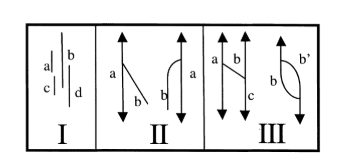
\includegraphics[width=0.5\textwidth]{Figuras/tipoFract-II.png}
\caption{Tipos de terminação de fratura. Fraturas isoladas (Tipo I, por exemplo, fratura $b$), fraturas conectadas individualmente (Tipo II, fratura $b$) e fraturas conectadas com outras fraturas em mais de um local (Tipo III, fraturas $b$ e $b'$) Fonte:~\protect\cite{ortega2000prediction}.}
\label{fig:tipoFraII}
\end{figure}

Singhal e Gupta~\cite{singhal2010applied} também destacaram que as fraturas podem ser identificadas em dois tipos: sistemática, que são planares e mais regulares na distribuição, e não-sistemática, que são irregulares e curvadas, como ilustra a Figura~\ref{fig:tipoFra}.

\begin{figure}[!htb]
\centering
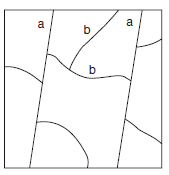
\includegraphics[width=0.2\textwidth]{Figuras/tipoFract.png}
\caption{Representação dos tipos de fratura. (a) sistemática e (b) não sistemática. Fonte:~\protect\cite{singhal2010applied}.}
\label{fig:tipoFra}
\end{figure}

\item A orientação da fratura, que pode ser classificada em vertical, horizontal e inclinada. Esta característica geralmente restringe as direções potenciais nas quais os fluidos podem fluir em um sistema de rochas fraturadas~\cite{fractfeature}.

\item A densidade da fratura que corresponde ao grau/intensidade de fraturamento da rocha, podendo ser descrita de três maneiras: linear, regional e volumétrica.

\begin{itemize}

\item A densidade de fratura linear é o número médio de fraturas de um determinado conjunto, sendo medido em uma direção perpendicular ao plano da fratura.

\item A densidade de fratura regional (densidade de fratura 2D) é uma maneira de quantificar a persistência da descontinuidade. Refere-se ao comprimento médio de traços por unidade de área em uma superfície plana.

\item A densidade de fratura volumétrica (densidade de fratura 3D) é a área de superfície fraturada média por volume de rocha unitária, criada por todas as fraturas de um determinado conjunto.

\end{itemize}

\end{itemize}

\section{Metodologia}
\label{sec:metodo}

Nesta seção, a metodologia desenvolvida para a execução dos métodos de fraturas e poros será descrita em detalhes. Inicialmente, a técnica de segmentação utilizada para ambos contextos será descrita e, em seguida, os métodos para a extração de características de forma individual. O métodos desenvolvidos foram aplicados em bases de dados públicas disponíveis na Internet.

\subsection{Segmentação}

A segmentação das imagens é realizada em duas etapas até se chegar ao resultado final. A primeira etapa é para criar uma máscara que indica a região de interesse da imagem, enquanto que a segunda etapa produz uma imagem referente ao conteúdo da rocha. Dessa forma, pela combinação desses resultados, pode-se criar uma imagem somente com as estruturas internas que serão usadas para as próximas análises.

Para a criação da máscara, aplicou-se uma série de técnicas de processamento de imagens que utilizam funções advindas da biblioteca \texttt{Scikit-Image}~\cite{scikit-image} e da biblioteca \texttt{OpenCV}~\cite{itseez2015opencv}.

\begin{figure}[!htb]
\centering
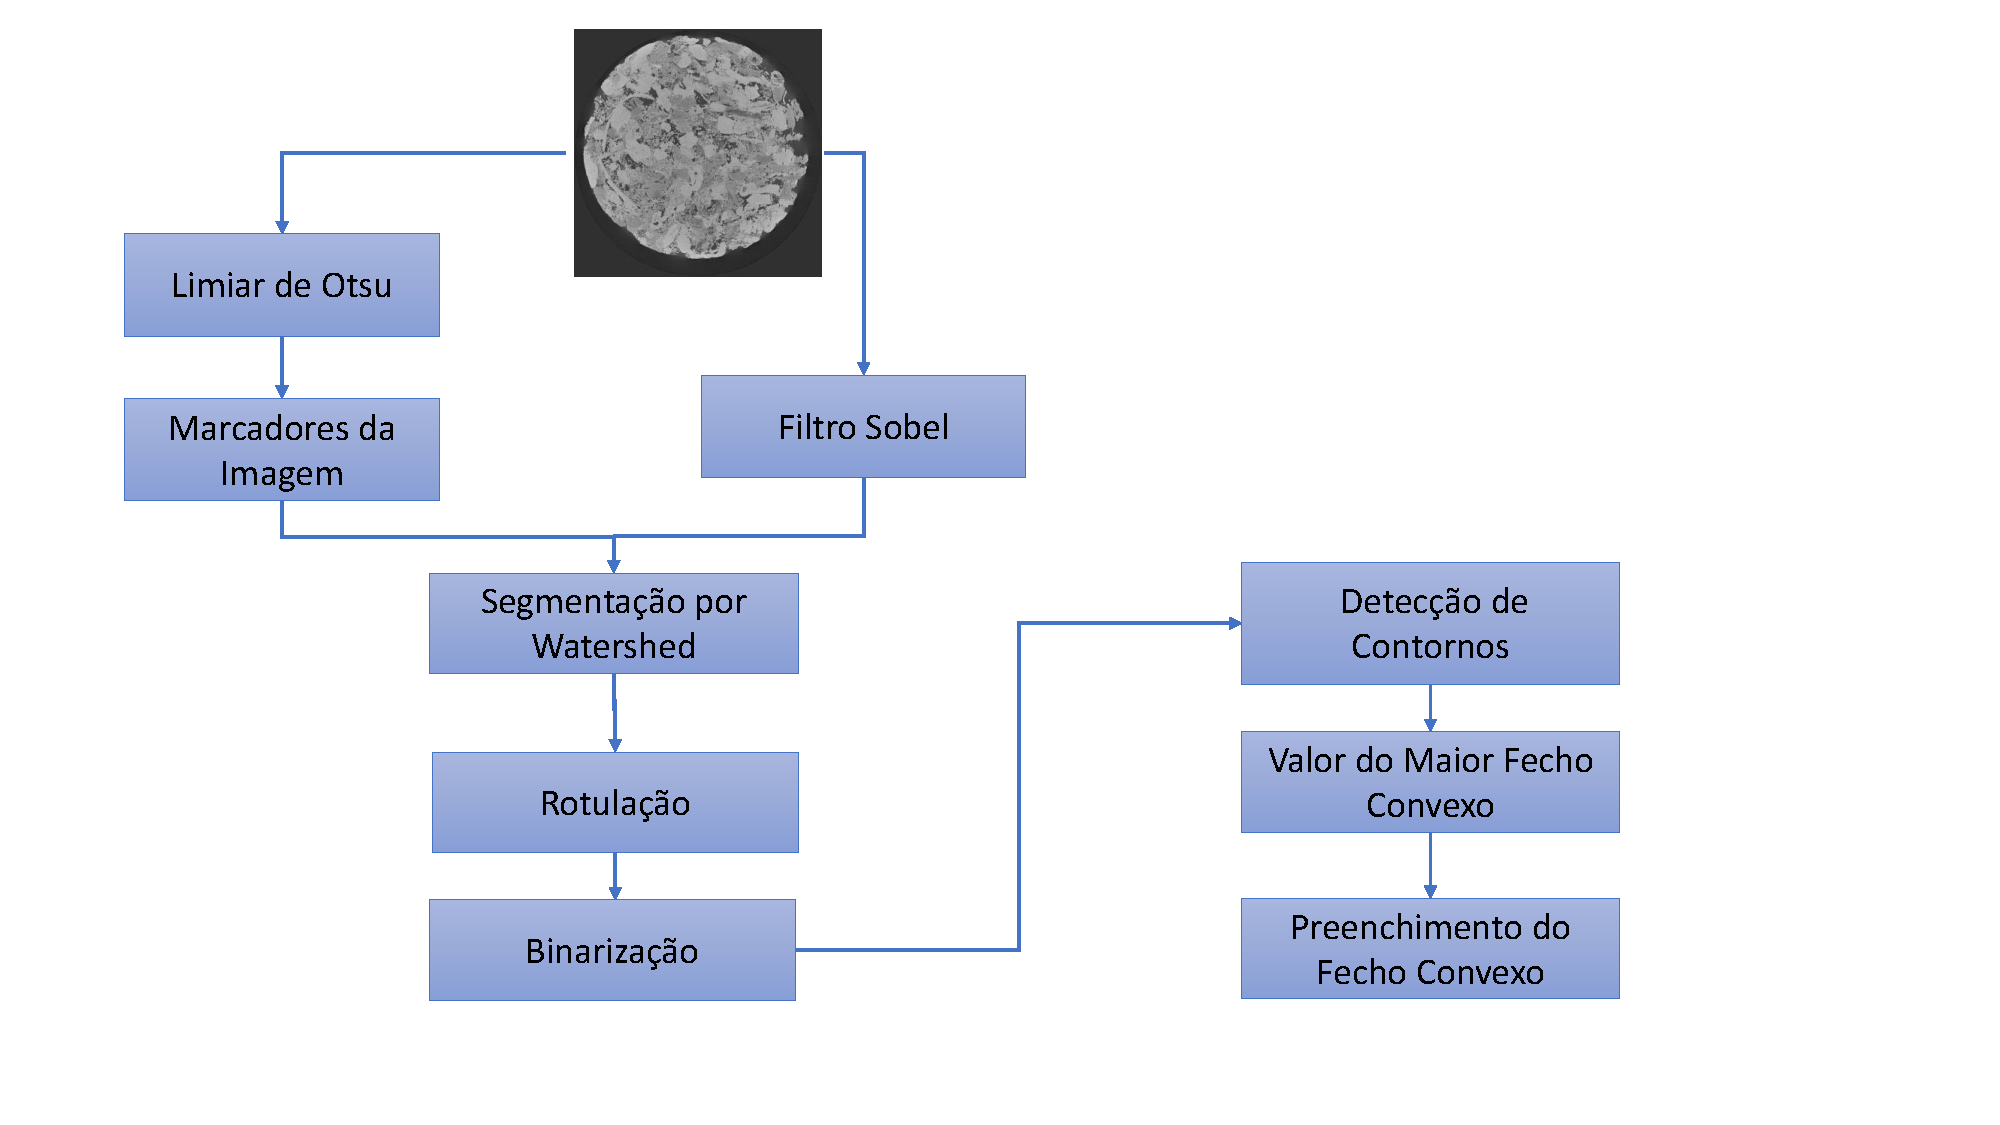
\includegraphics[width=0.6\textwidth]{Figuras/mtd-2.pdf}
\caption{Diagrama referente ao processo de segmentação.}
\label{fig:segmentacao}
\end{figure}

Na Figura~\ref{fig:segmentacao}, pode-se visualizar um diagrama que exemplifica o processo de aplicação desses algoritmos para a execução da segmentação. Nele, a segmentação incia com a aplicação da limiarização de Otsu na imagem original, para extrair o melhor limiar que separa as intensidades da imagem. Em seguida, uma imagem rotulada é criada com as regiões objeto/fundo separadas a partir do limiar obtido, utilizando-se o seguinte critério:
\begin{equation}
\textit{rótulo}(x) = \begin{cases}1, & \textit{se original}(x) < 30\\2,& \textit{se original}(x) > \textit{limiar de Otsu}\end{cases}\
\end{equation}

Também é necessária a criação de uma mapa de elevação, obtido através do filtro de Sobel, para ser usado como parâmetro da segmentação pela técnica de \textit{watershed} junto com a imagem rotulada. A criação desse mapa é um passo critico para uma boa segmentação e ajuda a definir as barreiras das estruturas da imagem.

Após esse procedimento, aplica-se a técnica de \textit{labeling} na imagem segmentada resultante a fim de marcar suas regiões e gerar um novo modelo binário, tal que:
\begin{equation}
\textit{binário}(x) = \begin{cases}0, & \textit{se labeling}(x) = 0\\255,& \textit{se labeling}(x) \neq 0\end{cases}\
\end{equation}

A partir desse resultado, em que a região de interesse da imagem está destacada, os contornos são detectados e é feita uma análise dos seus fechos convexos para extrair aquele que possuir maior tamanho, referindo-se ao polígono proporcionado pela área da rocha. Assim, a imagem da máscara é formada pelo preenchimento do maior fecho convexo, gerando uma saída com a área relativa à rocha em branco e o fundo dela em preto.

Este longo processo de segmentação é necessário pois a amostra da rocha costuma ter poros em sua borda, tal que uma simples binarização impossibilitaria a contagem e a extração da geometria desses poros, já que eles não teriam uma borda que os delimitassem, sendo dessa forma confundidos com o fundo, como mostra a terceira imagem na sequência apresentada na Figura~\ref{fig:img_segmentacao}. Assim, com a criação dessa máscara em formato circular englobando toda a área da amostra, todas as estruturas localizadas nessa região de interesse passam a ser contadas.
	
\begin{figure}[!htpb]
\centering
\subfloat[]{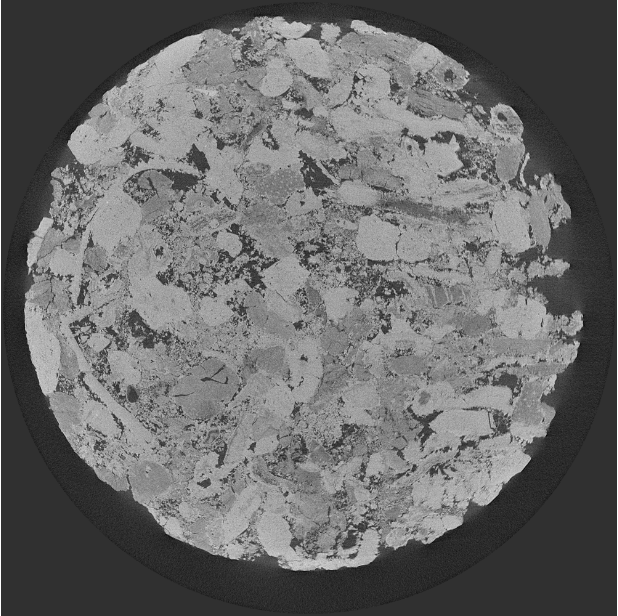
\includegraphics[width=0.11\textwidth]{Figuras/img_original.png}} \hspace*{0.1cm}
\subfloat[]{
\includegraphics[width=0.11\textwidth]{Figuras/mask.png}} \hspace*{0.1cm}
\subfloat[]{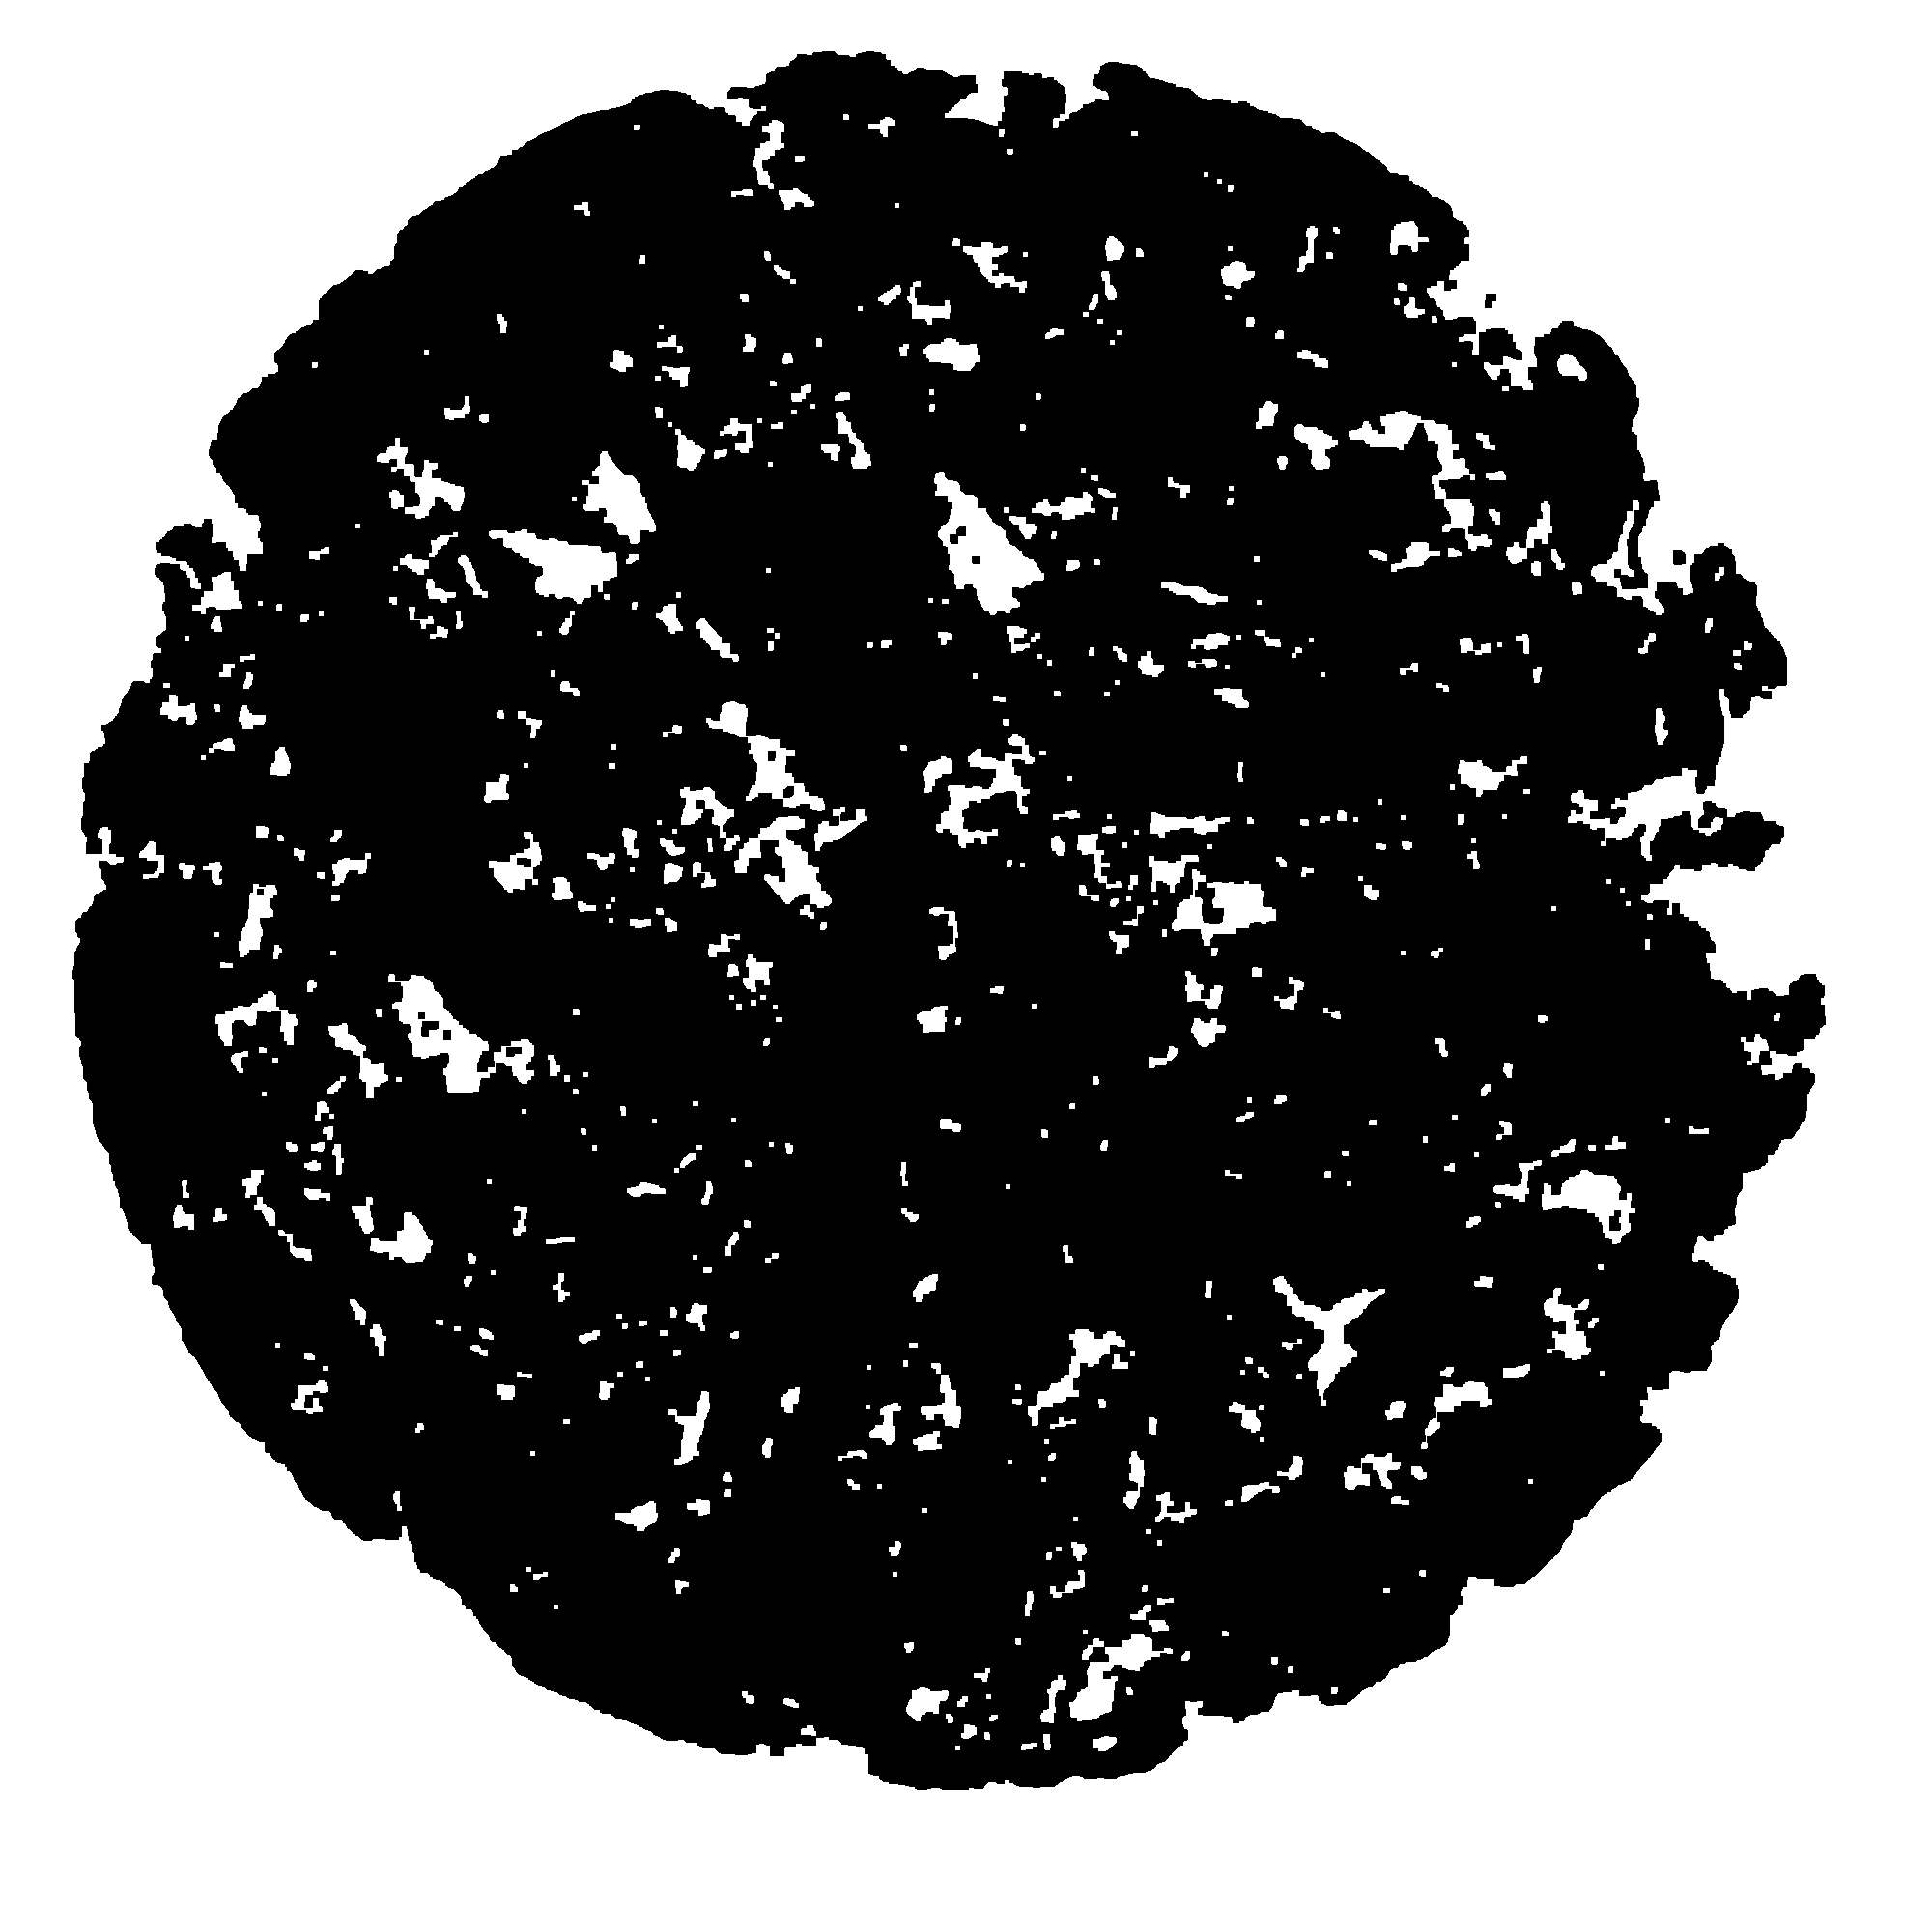
\includegraphics[width=0.11\textwidth]{Figuras/sure.png}} \hspace*{0.1cm}
\subfloat[]{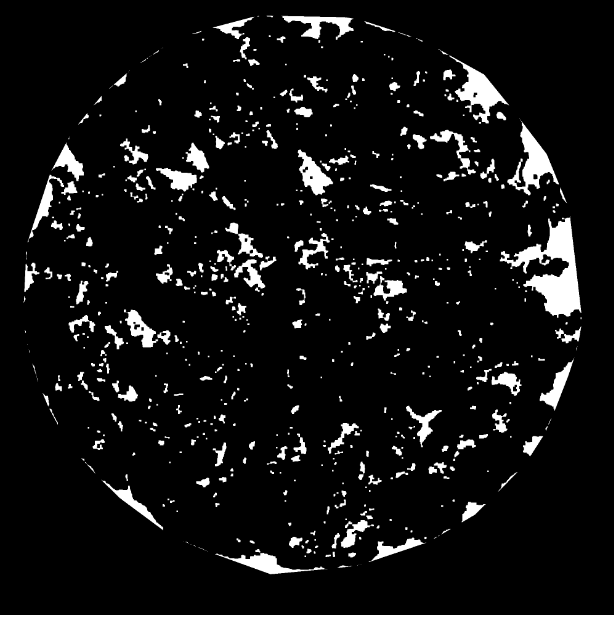
\includegraphics[width=0.11\textwidth]{Figuras/seg_final.png}}
\caption{Imagem de microtomografia e o resultado das segmentações. (a) imagem original, (b) imagem referente à mascara, (c) imagem pelo limiar de Otsu e (d) imagem resultante das duas anteriores.}
\label{fig:img_segmentacao}
\end{figure}

Depois da criação da máscara, outra imagem é criada por meio da segmentação da imagem original pelo limiar de Otsu, e ambas imagens, quando utilizadas juntas, fornecem uma maior confiança na captação dos poros e das fraturas. Um exemplo dessas duas técnicas pode ser visto na Figura~\ref{fig:img_segmentacao}. Ao final, uma última imagem é criada com base nas duas anteriores para proporcionar uma visão apenas dos poros/fraturas. Dessa forma, onde existir um pixel branco nas duas imagens, a da máscara e a limiarizada, a cor branca é inserida também na terceira imagem; caso contrário, a cor preta é inseridas.

\subsection{Extração das Características}

Após a segmentação da imagem, é necessário encontrar os contornos que foram extraídos da imagem original afim de analisar as suas características. Para isso, utiliza-se a função \textit{findcountours} da biblioteca \texttt{OpenCV}, onde passamos a imagem segmentada como parâmetro e ela retorna os contornos que foram identificados.

\begin{comment}
\begin{figure}[!htpb]
\centering
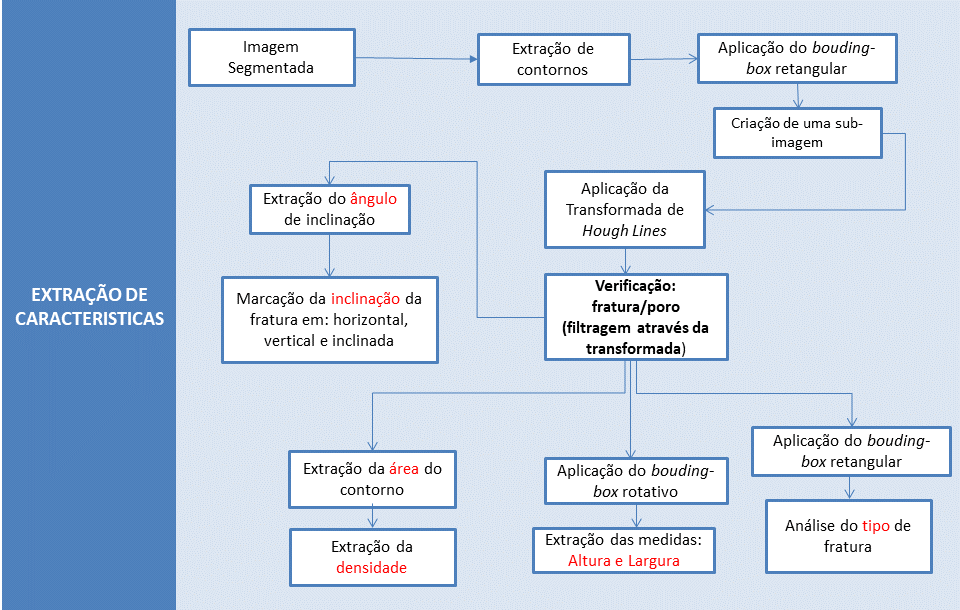
\includegraphics[width=0.5\textwidth]{Figuras/metodologia-algoritmoFraturas}
\caption{Metodologia do Algoritmo para analisar Fraturas.}
\label{fig:metodFracture}
\end{figure}
\end{comment}

Como a análise dos poros e fraturas é feita de forma separada, torna-se necessário fazer a identificação de cada um desses grupos. As fraturas possuem corpo alongado similar a uma reta, então utilizamos esse critério para fazer a separação. Uma forma de identificar essa característica é pela aplicação da Transformada de \textit{Hough Lines} em uma subimagem extraída pelo \textit{bounding-box} do corpo do contorno. Se for possível traçar uma reta, este contorno é classificado como uma fratura, senão ele é colocado de fora das próximas etapas. Na Figura~\ref{fig:houglines}, pode-se observar um exemplo do funcionamento desse processo aplicado em fraturas identificadas em uma amostra de carvão.

\begin{figure}[!htb]
\centering
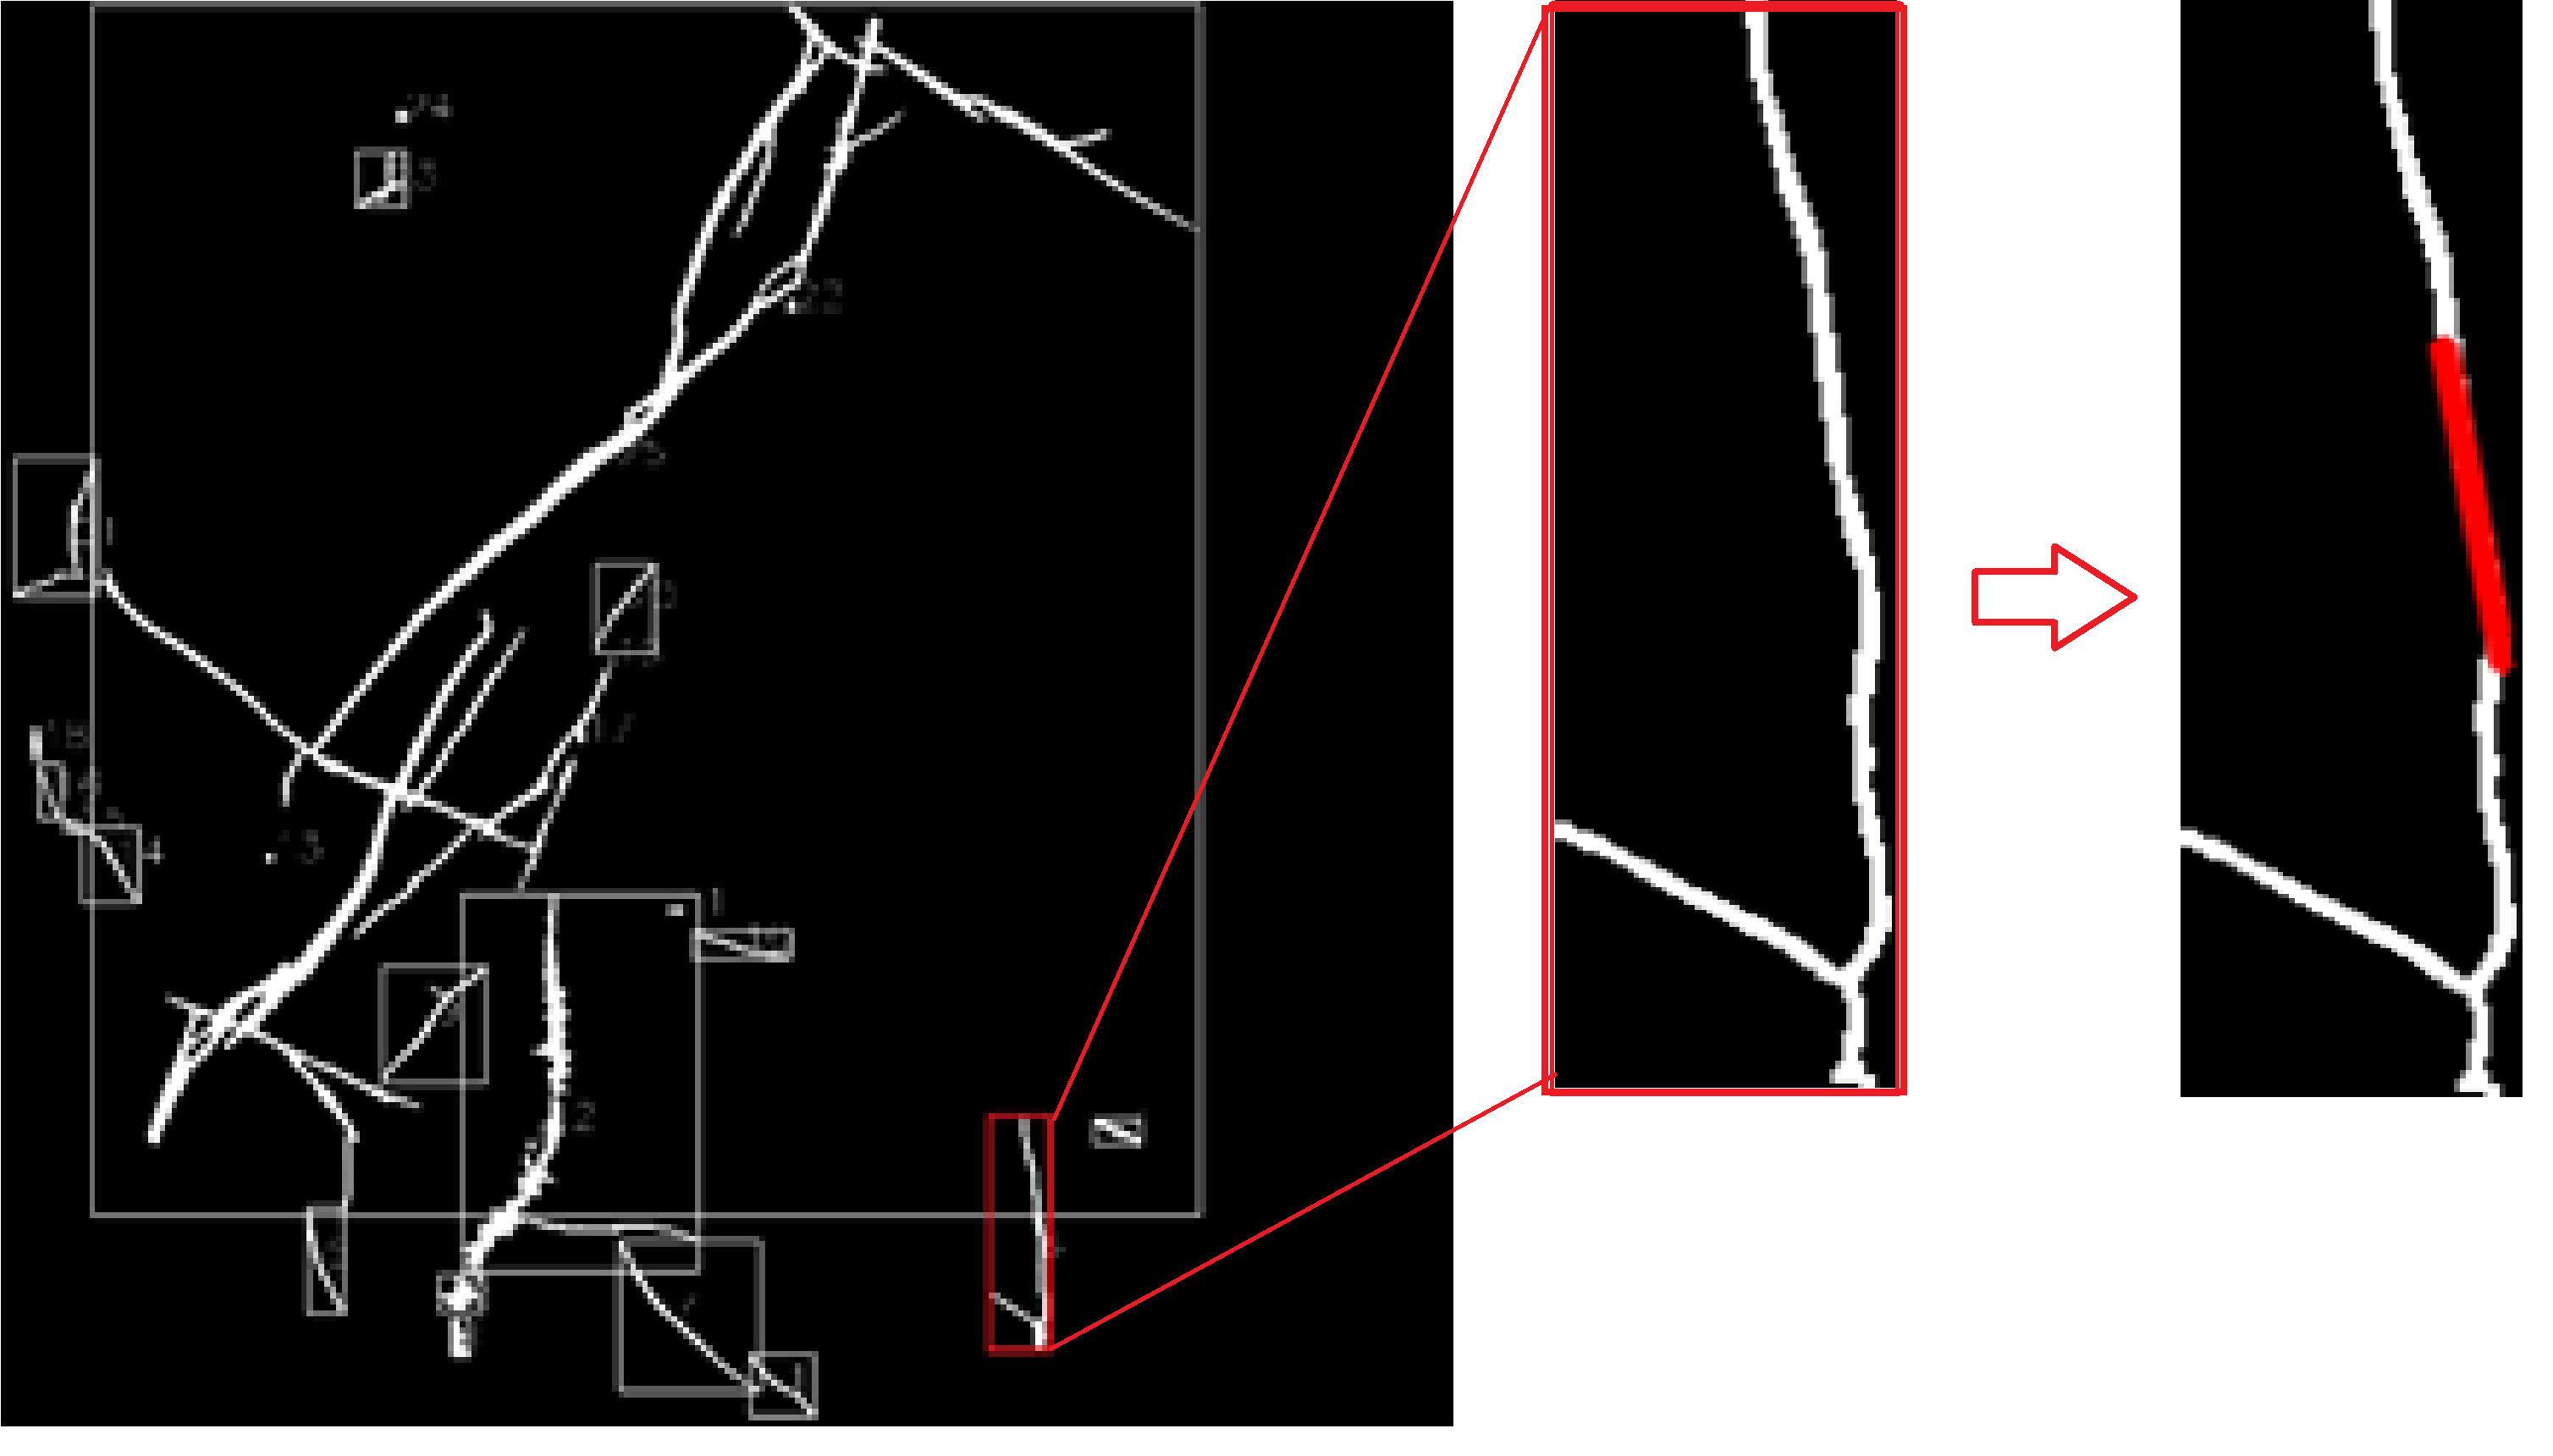
\includegraphics[width=0.45\textwidth]{Figuras/hough_lines.png}
\caption{Detecção de linhas pelo método de \textit{Hough Lines}.}
\label{fig:houglines}
\end{figure}

A partir dessa filtragem, as características descritas na Subseção~\ref{sec:referencial} são analisadas. A transformada de \textit{Hough Lines} além de permitir a identificação das fraturas, também possibilita calcular sua inclinação através da equação da distância entre dois pontos $(x1,y1)$ e $(x2,y2)$ em graus, dada por:

\begin{equation}
   angle = atan(\frac{y1-y2}{x1-x2}) * \frac{180}{\pi }
\end{equation}


Características tais como área, altura e largura podem ser obtidas através da mesma função que extrai o contorno, pois seu retorno comporta alguns dados a respeito da geometria do objeto. Já o cálculo das densidades foi baseado nos conceitos definidos na seção \ref{sec:estado_arte}, é obtido diretamente da fratura. Para a densidade linear é utilizado o número de fraturas pelo diâmetro da amostra de rocha,

\begin{equation}
    d1= \frac{numero\ de\ fraturas}{diâmetro}
\end{equation}

Na densidade 2D, fazemos seu calculo pela média da largura das fraturas pela área total da amostra, sendo:
\begin{equation}
    d2 = \frac{mean(largura\ das\ fraturas)}{area\ total\ da\ amostra}
\end{equation}

Por fim, a densidade 3D, que calcula a relação da área das fraturas pela área da amostra:
\begin{equation}
    d3= \frac{area\ total\ das\ fraturas}{area\ total\ da\ amostra}
\end{equation}


Para a caracterização da estrutura da fratura, por exemplo, sua conectividade e seu tipo, a análise deve ser mais sofisticada devido as suas particularidades, principalmente pelo fato de que muitas fraturas podem estar próximas e interferir em uma análise individual. Sendo assim, duas metodologias foram desenvolvidas para a definição desses critérios:

\begin{itemize}

\item Conectividade: a primeira forma desenvolvida de identificar as bifurcações das fraturas foi percorrer cada coluna do \textit{bounding-box} não rotativo de cada fratura em particular. Assim, nesse processo seria possível contar quantas transições ocorrem de intensidade relativa à fratura (branco) ao fundo da imagem (preto). Se houvesse mais de uma transição na mesma coluna, isto indicaria que haveria uma bifurcação, elevando seu tipo de classificação (Tipo I, II, III) a cada transição encontrada. Porém, como indica a Figura~\ref{fig:conectividade}, há uma série de fraturas que possuem partes de outras inseridas em seu \textit{bounding-box}, o que traz um resultado incorreto ao algoritmo desenvolvido. Com base no estudo de alguns métodos para identificação de componentes conexos (CC), aplicou-se a técnica de \textit{labeling} em que, a partir desse conceito, atribui um mesmo rótulo a um CC, tornando possível aplicar novamente o algoritmo inicial, mas dessa vez com as estruturas de um \textit{bounding-box} rotuladas. Dessa forma, a fratura de maior domínio recebe rótulo igual a 1 e o fundo da imagem recebe rótulo 0, possibilitando que as transições só sejam contadas quando ocorrerem entre esses dois valores. Assim, se no \textit{bounding-box} houver uma outra fratura, esta receberá outro rótulo, com o número 2 (sendo ilustrado com a cor azul), não interferindo no resultado.

\begin{figure}[!htb]
\centering
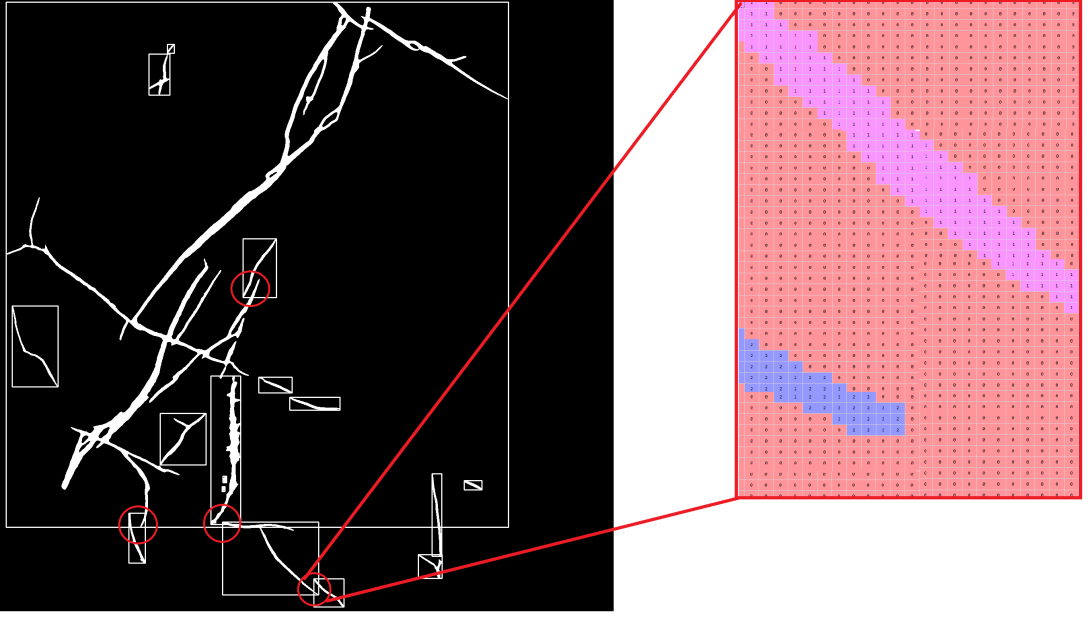
\includegraphics[width=0.5\textwidth]{Figuras/conectividade.png}
\caption{Identificação de componentes externos no \textit{bounding-box} de uma fratura}
\label{fig:conectividade}
\end{figure}

\item Tipo: Para a classificação da bifurcação, em termos de sistemática e não sistemática, aplicou-se uma segmentação com maior tolerância a ruído. Na imagem resultante, indicada na Figura~\ref{fig:ruidos}, pode-se observar que apareceram diversas fraturas pequenas e finas. Quando aplicados \textit{bounding-boxes} nesses contornos, percebeu-se que o valor correspondente à largura era bem baixo se a característica dele fosse sistemática. Assim, extraímos a largura de todas as fraturas e as ordenamos por ordem crescente a fim de identificar esse padrão de espessura do \textit{bounding-box} que excluiria a possibilidade de existir uma bifurcação.

\begin{figure}[!htb]
\centering
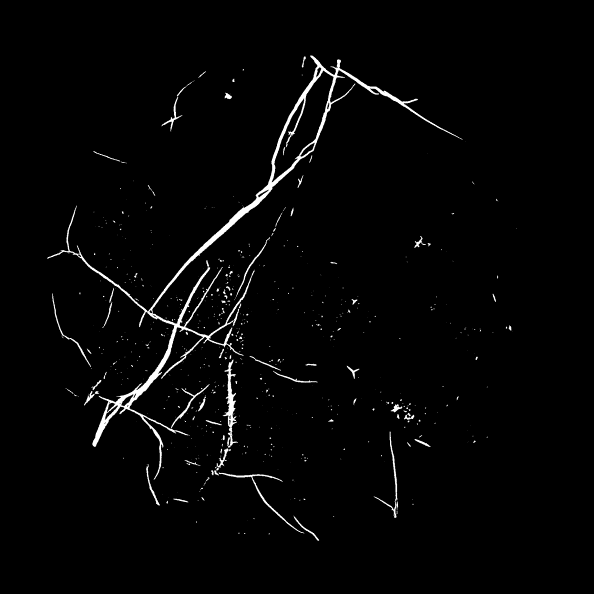
\includegraphics[width=0.25\textwidth]{Figuras/seg_ruidos.png}
\caption{Imagem segmentada com maior tolerância a ruídos.}
\label{fig:ruidos}
\end{figure}

A partir do gráfico mostrado na Figura~\ref{fig:grafico}, pode-se observar um aumento significativo quando a largura é maior do que 60. Dessa forma, a cada \textit{slice} analisado é calculada uma média de todos os valores abaixo desse limiar. O resultado é utilizado como parâmetro para classificar a fratura em sistemática, quando a largura é menor do que o limiar, ou não sistemática, quando maior.

\begin{figure}[!htb]
\centering
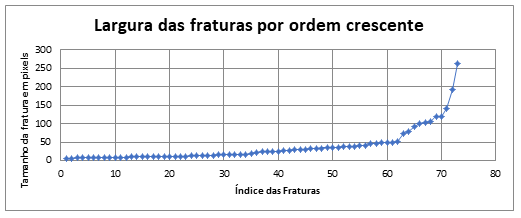
\includegraphics[width=0.5\textwidth]{Figuras/grafico_tamanho.png}
\caption{Gráfico da largura de todas as fraturas de um \textit{slice}.}
\label{fig:grafico}
\end{figure}

\end{itemize}

\subsection{Visualização 3D}

Para obter uma visualização completa das imagens segmentadas e compreender a distribuição das estruturas de interesse, implementamos uma função que permite a visualização 3D dessas amostras a partir da ferramenta VTK.

\begin{figure}[!htb]
\centering
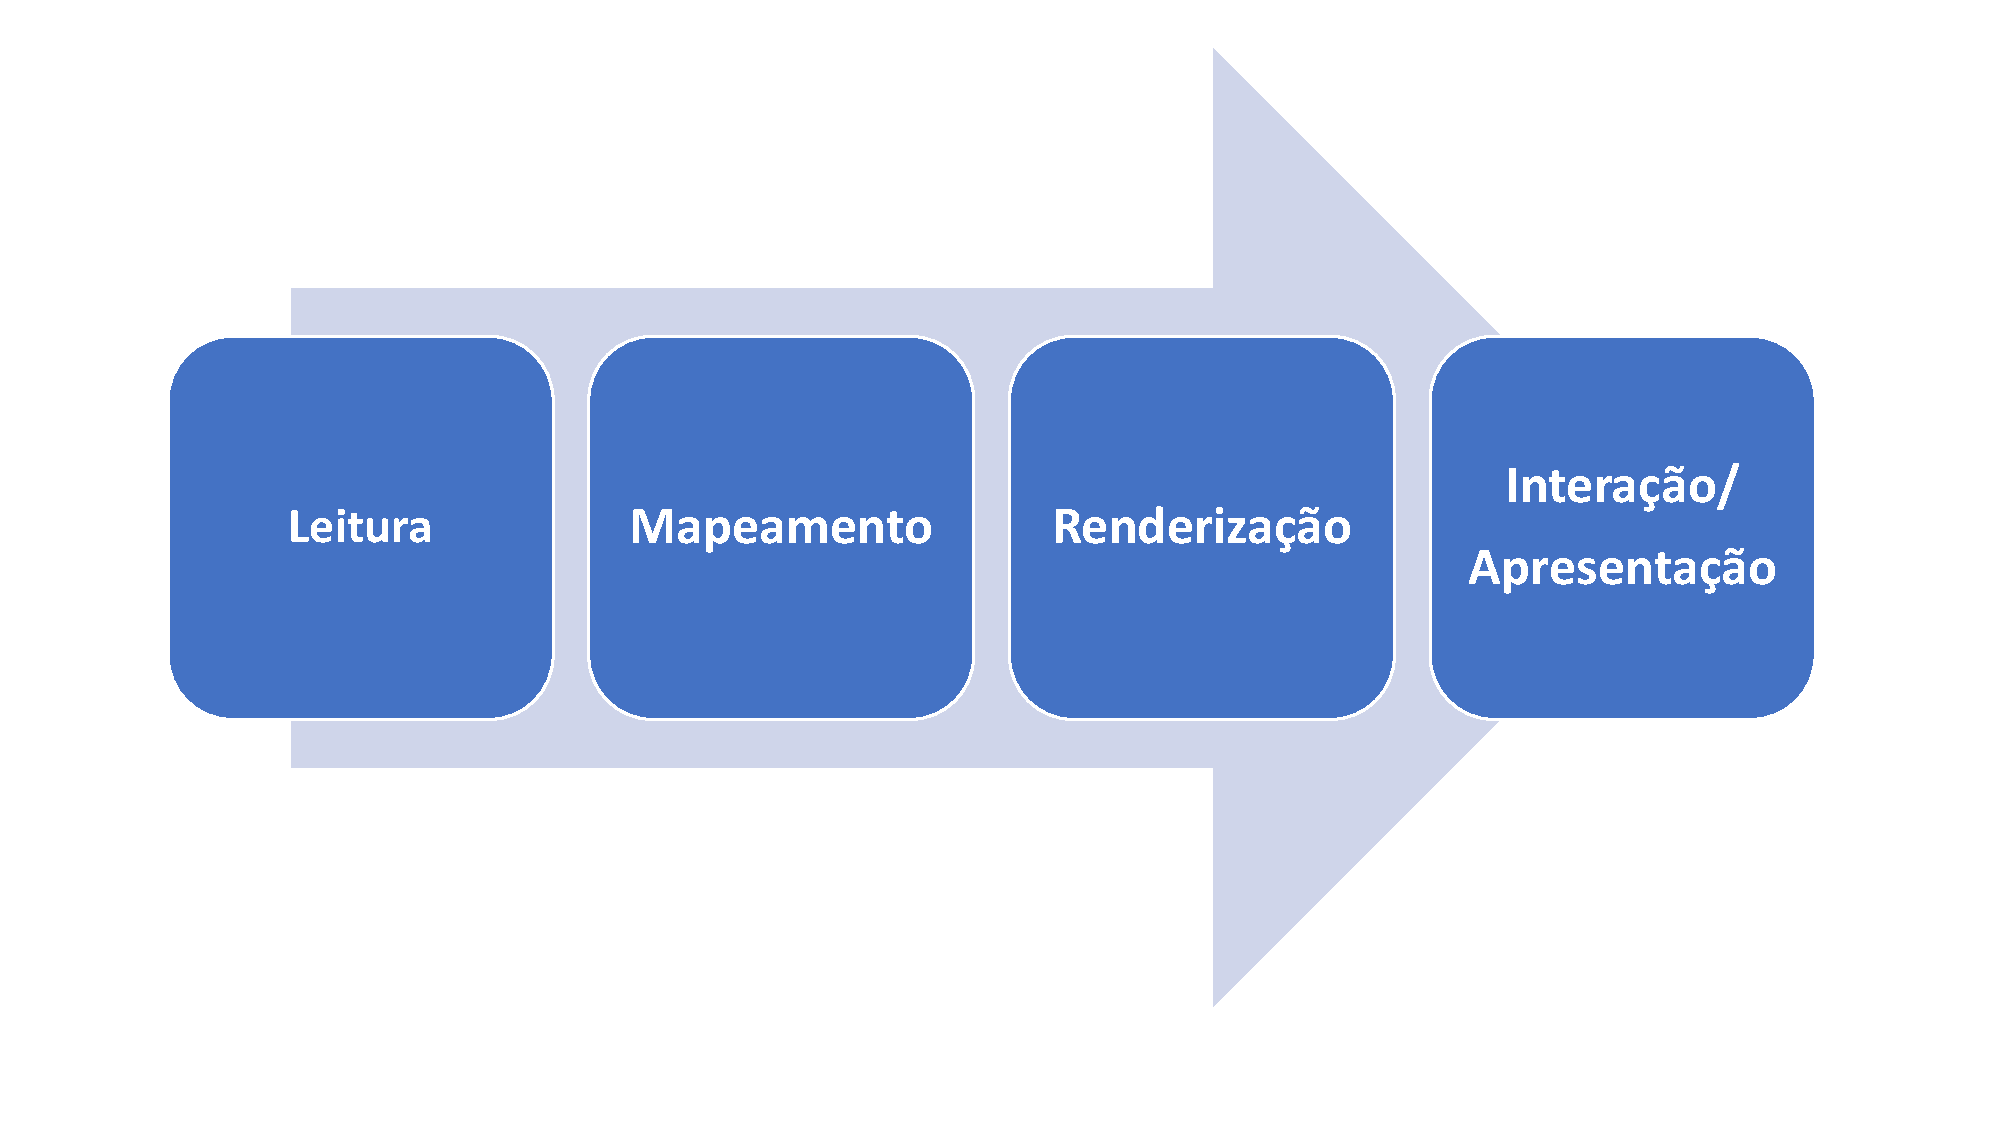
\includegraphics[width=.5\textwidth]{Figuras/fases_vtk.pdf} \hspace*{0.1cm}
\caption{Fluxo da construção do modelo de visualização.}
\label{fig:fluxo_vtk}
\end{figure}

O VTK permite a leitura das imagens em formato TIFF por meio da classe \texttt{vtkTIFFReader()}. Após a leitura das imagens, definimos uma função de transferência para mapear uma propriedade (nestes casos, um valor escalar) para um valor de cor {\it Red-Green-Blue} (RGB) pela classe \texttt{vtkColorTransferFunction()}. Definimos também a característica de opacidade que permitirá que apenas as estruturas em branco sejam visualizadas, enquanto a cor preta da imagem seja descartada pela adição da transparência.

Em seguida, um mapeamento eficaz do volume é gerado no espaço 3D pela classe \texttt{vtkSmartVolumeMapper()} e adicionado à tela de renderização. Com o intuito de prover uma experiência interativa do usuário e a amostra, integramos a esta tela um objeto interativo da classe \texttt{QVTKRenderWindowInteractor()}, que permite que o usuário tenha diferentes visões da amostra pelos movimentos realizados com o {\it mouse} ao pressionar o objeto renderizado.

\section{Resultados}
\label{sec:resultados}

Como resultado da elaboração dos modelos de análise das estruturas internas de rochas, desenvolvemos uma interface que promove a interação do usuário com os dados obtidos através da implementação dos métodos descritos na seção anterior. Dessa forma, foram criados dois diferentes ambientes para cada propósito, em que todos os resultados podem ser analisados qualitativamente.

Para uma maior compreensão da escala real desses dados, uma transferência de métricas pixels-milímetros pode ser feita a partir da interação do usuário com a interface ao indicar o valor que o pixel corresponde; caso esse dado seja desconhecido, pode ser inserido o valor 1 e o resultado será em pixels.

Na área desenvolvida para as fraturas, mostrada na Figura~\ref{fig:TelaFratura}, todos os dados do processamento são visualizados. Estes dados podem ser alterados através da \textit{SliceBar}, onde o usuário poderá escolher sobre qual \textit{slice} ele deseja visualizar as informações. Assim, após o usuário enviar o bloco de \textit{slices} correspondente a sua amostra, duas imagens são exibidas na tela, uma referente à imagem original e outra referente à segmentação, do primeiro \textit{slice} do bloco.

\begin{figure}[!htb]
\centering
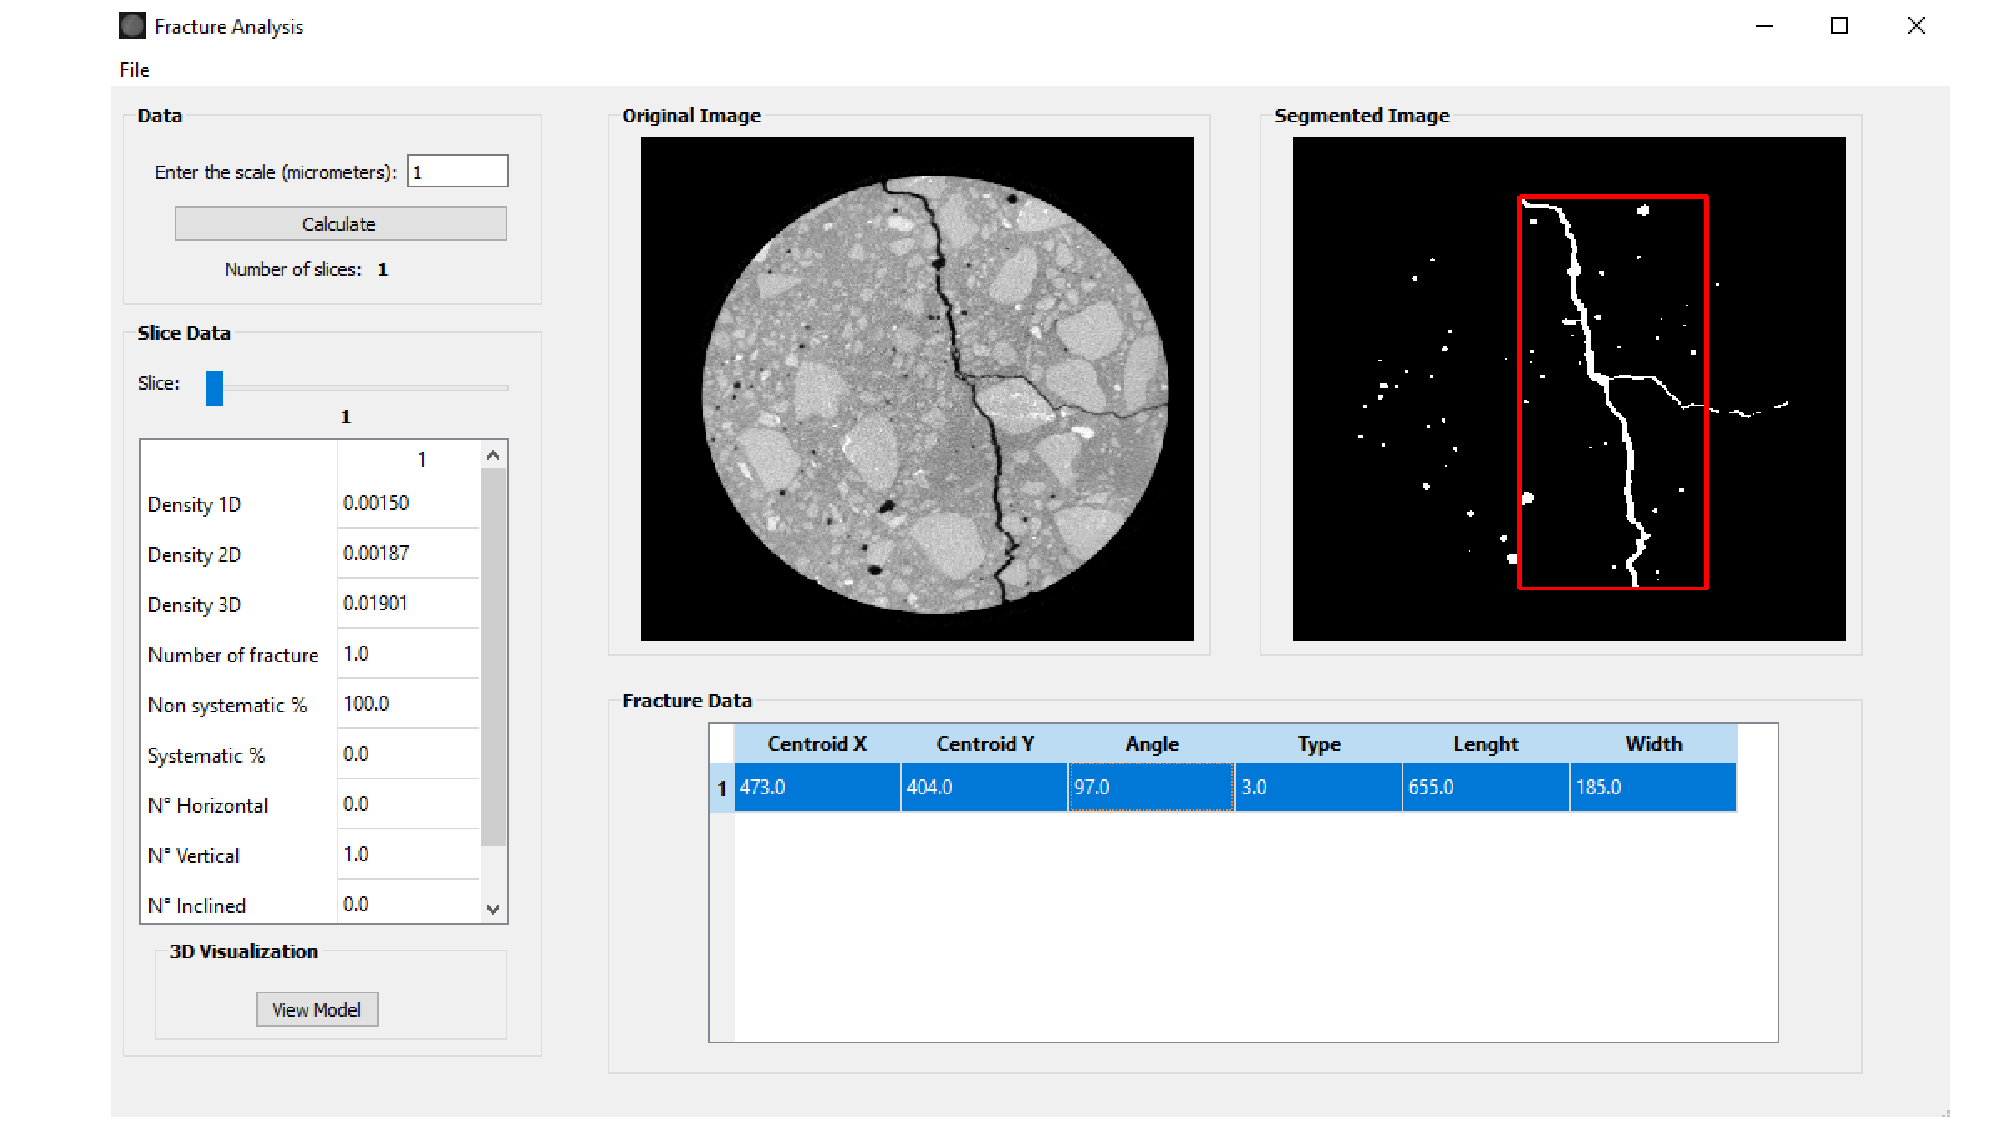
\includegraphics[width=0.5\textwidth]{Figuras/tela-fracture.pdf}
\caption{Tela da interface para analisar e visualizar as fraturas.}
\label{fig:TelaFratura}
\end{figure}

Juntamente com as imagens, também são exibidos os dados das fraturas em duas tabelas. Na tabela vertical, encontram-se os dados que correspondem ao \textit{slice} como um todo, destacando as seguintes características: a quantidade de fraturas no \textit{slice}, as densidades do \textit{slice} (1D, 2D e 3D), o número de fraturas verticais, horizontais e inclinadas, e a percentagem de fraturas sistemáticas e não sistemáticas. Já na tabela horizontal, localizada abaixo das duas imagens, pode-se ver os dados de cada fratura, sendo indicados pelas linhas da tabela. Para uma melhor correspondência dos números com as imagens, ao clicar nas linhas da tabela, o usuário pode ver, na imagem segmentada, uma marcação na fratura à qual aquele dado se refere.

Por fim, é possível obter a visualização 3D dos \textit{slices} de entrada, onde o usuário pode interagir visualizando sua amostra de diferentes ângulos, como ilustrado na Figuras~\ref{fig:tela3DFraturas}.


\begin{figure}[!htb]
\centering
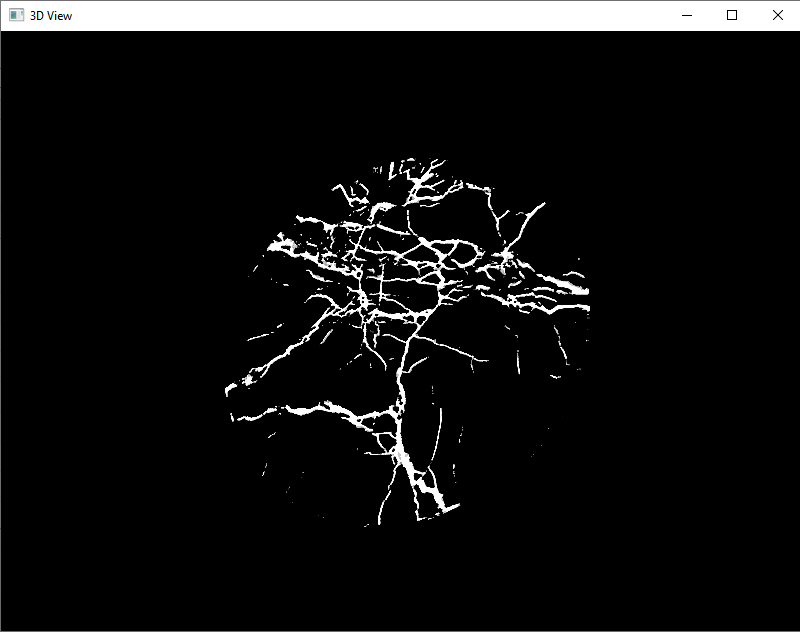
\includegraphics[width=0.22\textwidth]{Figuras/F-3dview-1.png}
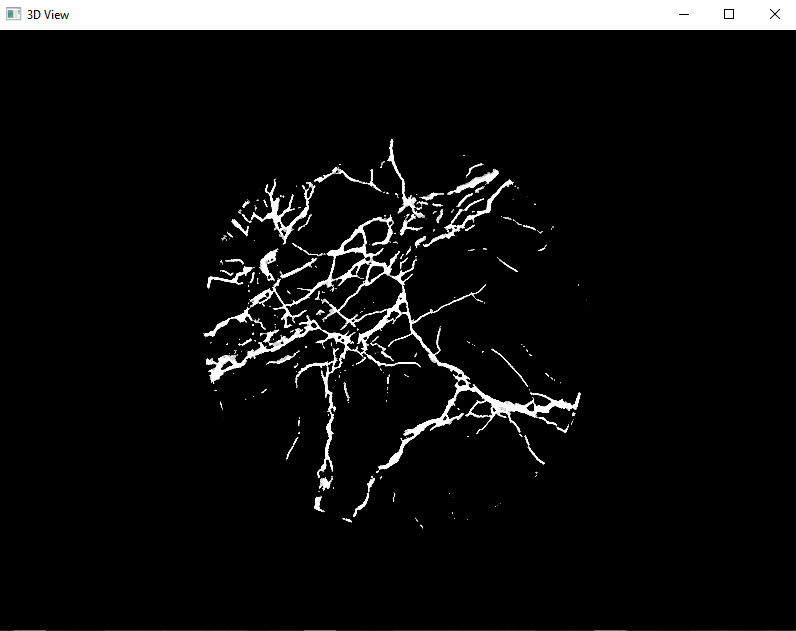
\includegraphics[width=0.22\textwidth]{Figuras/F-3dview-2.png}
\caption{Diferentes visões obtidas por 5 \textit{slices}, passados como entrada, na tela de visualização 3D.}
\label{fig:tela3DFraturas}
\end{figure}

Para indicar como o usuário pode interagir com o sistema, um diagrama de casos de uso, indicado na Figura~\ref{fig:casos-2}, foi desenvolvido. Assim, como descrito, para calcular as métricas a respeito das fraturas o usuário necessita primeiramente carregar as imagens das quais deseja obter a análise, e inserir a escala referente ao diâmetro da amostra (em milímetros). A partir disso, os resultados são exibidos e o usuário pode realizar a visualização 3D da amostra, alterar as fatias em exibição e também selecionar,na tabela de fraturas, uma fratura para ser destacada na imagem segmentada

\begin{figure}[!htb]
\centering
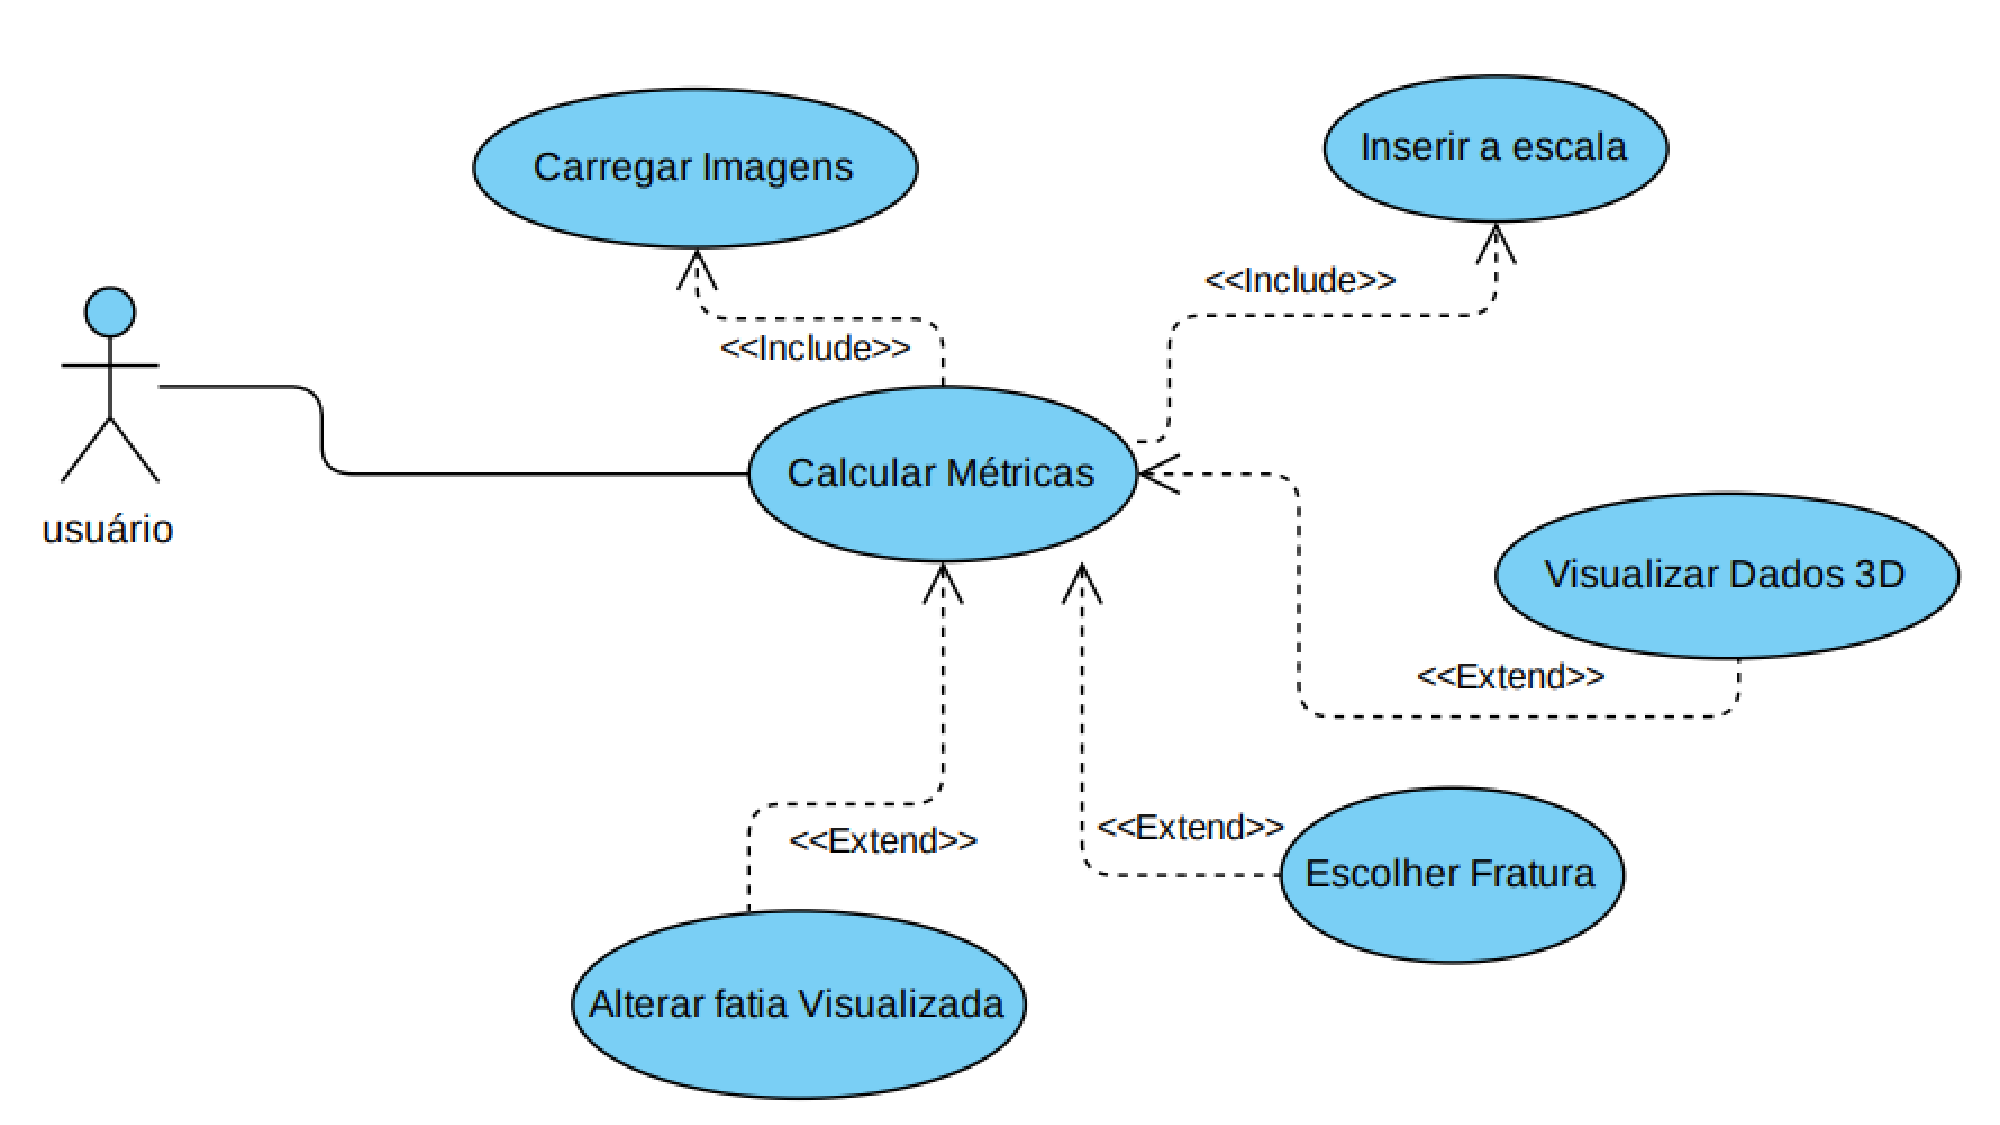
\includegraphics[width=8cm]{Figuras/casos-2.pdf}
\caption{Diagrama de casos de uso da análise de fraturas.}
\label{fig:casos-2}
\end{figure}



\section{Conclusões}
\label{sec:conclusoes}

Este artigo visou apresentar uma ferramenta complementar para os pesquisadores que atuam com o manuseio de imagens advindas de microtomografia computadorizada de rochas. Nesse sentido, pode-se oferecer um ambiente em que os poros e as fraturas possam ser identificados e descritos, trazendo uma análise sobre seu comportamento e forma, a fim de contribuir para uma avaliação não-destrutiva de amostras que representam um conjunto em estudo.

Propostas para trabalhos futuros podem ser desenvolvidas a fim de proporcionar um aprendizado na identificação da presença de fratura nas imagens porosas e, assim, encaminhar, quando detectadas, para a análise geométrica.

\section*{Agradecimentos}
\label{sec:agradecimentos}

Os autores gostariam de agradecer o suporte financeiro provido pela Fundação de Amparo à Pesquisa (FAPESP), processo 2017/50065-2, com o autor sob número 2018/01439-0, e pela Coordenação de Aperfeiçoamento de Pessoal de Nível Superior (CAPES).

\bibliographystyle{unsrtnat.bst}
\bibliography{Artigo.bib}

\end{document}
